\chapter{ctexbook使用简介}
\label{chap:ctexbook}

中文文档类测试。你需要将所有源文件保存为 UTF-8 编码。
你可以使用 XeLaTeX、LuaLaTeX 或 upLaTeX 编译,也可以使用 (pdf)LaTeX 编译。
推荐使用 XeLaTeX 或 LuaLaTeX 编译。对高级用户,我们也推荐使用 upLaTeX 编译。



\section{代码}
\index{代码}


下面是一段Python代码:
\begin{lstlisting}[language=python, caption={Python代码示例}]
def hello_world():
    print("Hello, World!")
\end{lstlisting}


\section{数学公式}
\index{数学公式}
\index{Attention}

我们可以通过公式\ref{attention_equation}来定义Attention。
\begin{equation}\label{attention_equation}\index{transformer}
    Attention(Q, K, V) = softmax(\frac{QK^T}{\sqrt{d_k}})V
\end{equation}

这里通过\texttt{\textbackslash label}来标识公式,通过\texttt{\textbackslash ref}来引用公式。

\section{引用文献}
\index{文献}
引用一个文献\cite{siffer2017anomaly}。


\section{图片}
插入PDF矢量图:

\begin{figure}[htbp]
    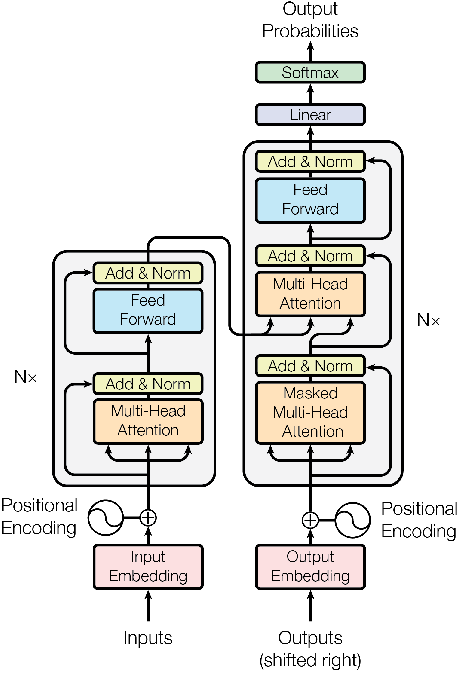
\includegraphics[width=0.6\textwidth]{./figures/transformer.pdf}
    \centering
    \caption{Transformer架构\cite{vaswani2017attention}}
    \index{transformer}
\end{figure}
